\chapter{Foundations}\label{ch:foundations}

This chapter introduces the technical foundations required for the remainder of the thesis. It first explains how diffusion models generate images, how latent diffusion improves efficiency by operating in a compressed representation rather than directly in pixel space, and how text prompts are encoded to guide the generation process. It then distinguishes between the two representations used throughout this work: a detailed conditioning representation for image generation and a compact embedding for comparison, projection, and analysis. The remaining sections present the methods used to make these compact representations inspectable.

\section{Diffusion and latent diffusion basics}\label{sec:2.1}

Generative models aim to learn a data distribution so that new samples can be produced that resemble the observed data. Several different architectural approaches exist for this purpose. For this thesis, diffusion-based models are the most relevant because they currently form a major foundation of modern text-to-image systems.

Diffusion models generate data by reversing a noising process. In the forward process, noise is gradually added to a data sample over many steps until the signal is strongly degraded. In the reverse process, a neural network is trained to predict how this noise should be removed step by step, so that a new sample can be reconstructed from random noise. This makes generation iterative. Instead of producing the final image in one pass, the model refines an intermediate representation through a sequence of denoising updates, as illustrated in \hyperref[fig:diffusion-denoising-process]{Figure~\ref*{fig:diffusion-denoising-process}}. \cite{ho2020denoising}

\begin{figure}[htbp]
\centering
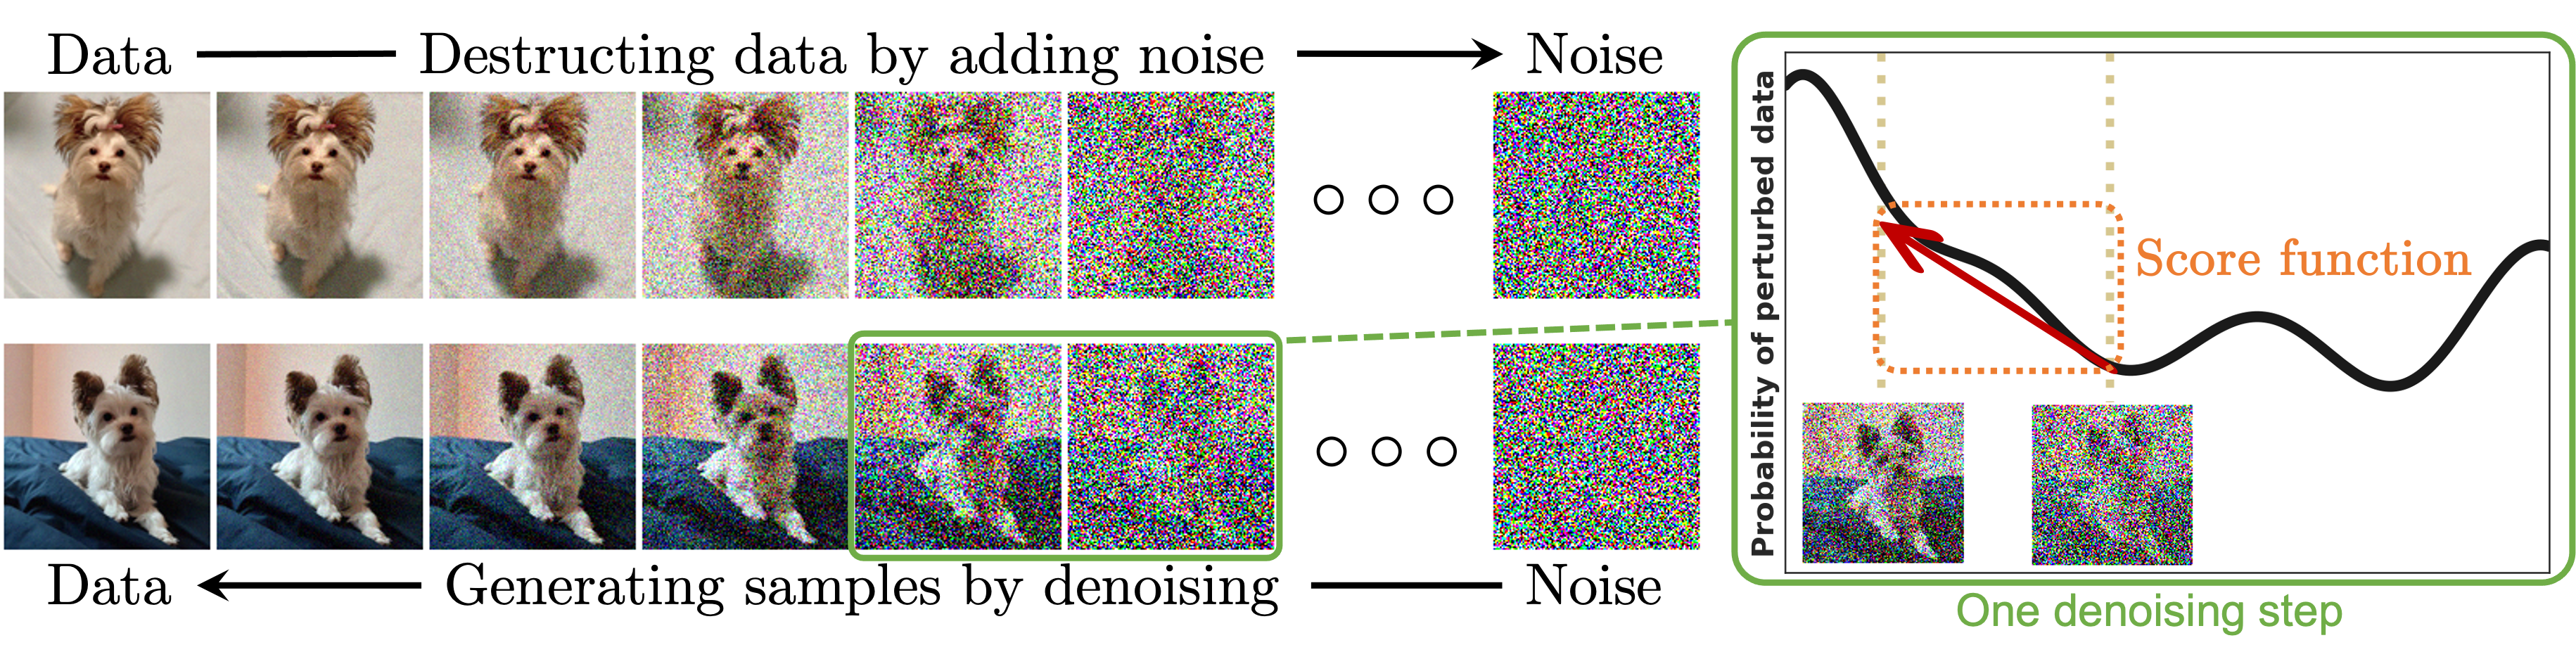
\includegraphics[width=0.9\textwidth]{figures/diffusion-denoising-process.png}
\caption{Illustration of the forward noising and reverse denoising process in diffusion models, from \cite{yang_diffusion_2025}, p.~6}
\label{fig:diffusion-denoising-process}
\end{figure}

This setup has two important consequences. First, diffusion models are flexible and can be conditioned in different ways, for example through text. Second, they are computationally expensive when they operate directly in pixel space, because the model has to process high-dimensional image tensors repeatedly over many steps. This motivates the move from pixel-space diffusion to latent diffusion. \cite{rombach2022latent}

Latent diffusion models reduce this cost by applying the diffusion process in a compressed latent representation instead of directly on RGB images. The image is first encoded into a lower-dimensional latent space by an autoencoding model, then diffusion is performed in that latent space, and finally the result is decoded back into image space. This setup keeps much of the perceptually relevant structure while making training and sampling more efficient. The underlying autoencoding principle is related to latent-variable models such as variational autoencoders, which learn a continuous latent representation together with a decoder that reconstructs data in the original space. This learned encoder-decoder pair is what makes the reduction to a lower-dimensional space described above possible in the first place, since it must preserve enough information to reconstruct the original data despite the compression. \cite{rombach2022latent,kingma2014vae}

In text-to-image diffusion models, several distinct representation spaces coexist, making it misleading to refer to a single latent space. During the generation process, these representation spaces include the initial noise or seed space, the timestep-dependent denoising states, the autoencoder's compressed image-latent space, the prompt-embedding space used for conditioning, and the internal feature spaces of the denoising network \cite{rombach2022latent,samuel2023normguided,park2023riemannian,kwon2023semantic}. These spaces are not interchangeable, because they support different forms of variation, control, and interpretation.

\section{Conditioning, prompt embeddings, and CLIP-based text representations}\label{sec:2.2}

The relevant point here is that text-to-image diffusion relies on several interacting representational layers rather than on one undifferentiated latent space. Prompt conditioning is one of the most important space of these layers and therefore needs to be understood before latent-space exploration methods can be described precisely.

Conditioning means that generation is guided by additional information beyond random noise. In text-to-image generation, the most common conditioning input is a text prompt. The prompt is transformed into a representation that the diffusion model can process during denoising, so that the generated image becomes aligned with the given description. \cite{rombach2022latent}

An important background for such text representations is CLIP (Contrastive Language-Image Pre-training). Radford et al. introduce CLIP as a contrastive model that learns image and text encoders jointly from large numbers of image-text pairs. The text encoder maps natural-language input into an embedding space that is aligned with image representations. This makes CLIP-based text representations useful not only for retrieval or classification, but also as a general semantic representation of prompts. \cite{radford2021clip}

In text-to-image diffusion systems, prompt conditioning is typically richer than a single global sentence embedding. Latent diffusion models use cross-attention, which lets token-level text information influence the denoising process at multiple spatial locations and multiple steps. In other words, the prompt is not only represented once at the beginning. Its encoded content is repeatedly used while the image is being generated. \cite{rombach2022latent}

Recent work also shows that text embeddings are not merely passive inputs. They can themselves function as a semantically meaningful control space. Yu et al. show that manipulations in text embedding space can support controlled edits and reveal interpretable semantic directions, which means that prompt embeddings are not only technical carriers of text but also structured semantic representations \cite{yu2024textembedding}. Na et al. extend this perspective further by showing that a fixed prompt embedding cannot maintain optimal text-image alignment throughout the whole denoising process, since the image evolves at each step and the embedding that best matches it can therefore change over time. In DATE (Diffusion Adaptive Text Embedding), text embeddings are updated during sampling so that the conditioning can adapt to the intermediate image state and maintain this stronger text-image alignment \cite{na2025date}.

Consequently, prompt embeddings serve two distinct purposes in this work. First, they form part of the conditioning mechanism that directly guides image generation. Second, they provide an analytical representation that can be reduced or transformed for comparison, projection, clustering, and navigation.

\section{Compact embeddings versus real conditioning}\label{sec:2.3}

Building on the double role introduced above, this section defines the two sides of that distinction precisely. Real conditioning refers here to the full prompt-dependent representation that directly participates in image generation, and it is contrasted in this thesis with compact embeddings.

Compact embeddings serve a different purpose. They reduce prompts or intermediate representations to fixed-size vectors that can be stored, compared, searched, projected, clustered, and navigated efficiently. This makes them well suited to exploratory analysis and visualization. However, because this reduction discards part of the information contained in the full conditioning pathway, compact embeddings are not generatively equivalent to real conditioning and should not be treated as direct substitutes for it.

The plugin therefore relies on compact embeddings for comparison and interaction, while the produced images still depend on the model's richer internal conditioning structures.
Once such compact representations are available, the next question is how they can be transformed into a form that supports visual inspection and interactive exploration.

\section{Dimensionality reduction with UMAP / Parametric UMAP}\label{sec:2.4}

For this purpose, dimensionality reduction is used: a high-dimensional representation is projected into a lower-dimensional space that is easier to inspect, visualize, and analyze.

UMAP (Uniform Manifold Approximation and Projection) is a manifold-learning method for dimensionality reduction. It maps high-dimensional data, such as image or text embeddings, into a lower-dimensional space while aiming to preserve important local relations. The method is based on the assumption that the data lies approximately on a manifold. In a first step, UMAP identifies which points lie close to each other in the original high-dimensional space and represents these local relations as a weighted k-nearest-neighbor graph, whose edge weights describe how strongly points are connected within their local neighborhood.
In a second step, UMAP creates a low-dimensional representation of this graph. It arranges the points so that the neighborhood relationships of the original high-dimensional space are preserved as closely as possible. Strongly connected points should therefore remain close in the projection, whereas weakly connected or unrelated points should be positioned farther apart. The final layout is obtained by minimizing the difference between the graph defined in the original space and the graph induced by the low-dimensional representation. \cite{mcinnes2020umap}

A fitted UMAP model can also be used to project new data points into an existing embedding space. However, this transformation is still an approximation based on the learned neighborhood structure and the existing reference data. Nevertheless, this makes standard UMAP useful for adding new points after fitting, but repeated use in a runtime workflow can involve additional overhead and computation costs, because the transformation remains tied to the fitted structure. This overhead scales poorly as the reference dataset grows, since each new projection must be computed against the entire existing set of points.

Parametric UMAP is based on the same underlying objective as standard UMAP but represents the projection differently. Rather than optimizing the low-dimensional coordinates of individual samples directly, it trains a neural network to approximate the mapping from the original feature space to the reduced embedding space. Once trained, this network can project previously unseen data through a forward pass, making the method particularly suitable for workflows in which new prompts, images, or derived embeddings must be added repeatedly after the initial fit. \cite{sainburg2021parametricumap}

To summarize this section, UMAP is used here as the main method for projecting high-dimensional embeddings into lower-dimensional spaces, especially two and three dimensions (\hyperref[fig:umap-example-2d]{Figure~\ref*{fig:umap-example-2d}} and \hyperref[fig:umap-example-3d]{Figure~\ref*{fig:umap-example-3d}}), so that the latent space can be visualized and explored. These projections are useful for examining the mentioned local neighborhoods, cluster tendencies, and relationships between samples. Both standard UMAP and Parametric UMAP projections should nonetheless be interpreted as approximate views of the original structure rather than as exact geometric representations of distances in the high-dimensional embedding space.

\begin{figure}[htbp]
\centering
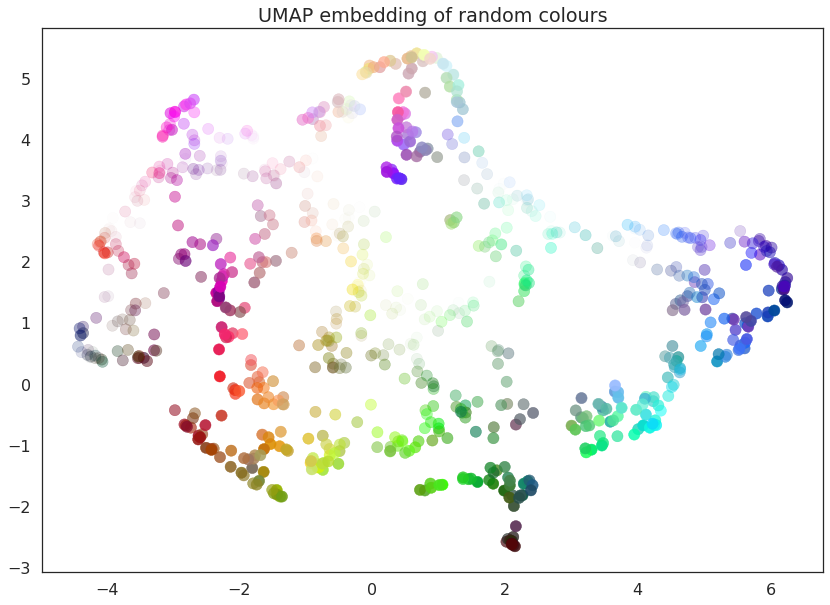
\includegraphics[width=0.5\textwidth]{figures/umap-example-2d.png}
\caption{UMAP embedding of random RGBA colors into 2 dimensions; nearby points share similar colors, from \cite{mcinnes2026umapparameters}}
\label{fig:umap-example-2d}
\end{figure}

\begin{figure}[htbp]
\centering
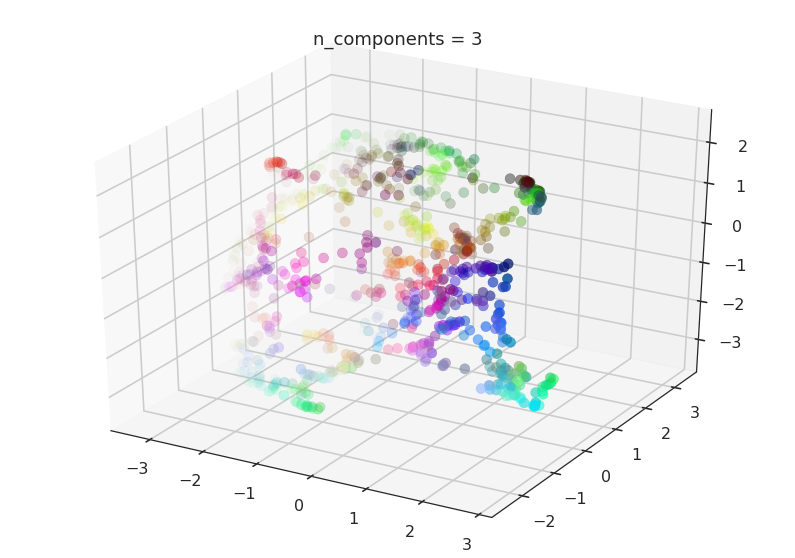
\includegraphics[width=0.5\textwidth]{figures/umap-example-3d.png}
\caption{The same random-color data embedded into 3 dimensions instead, from \cite{mcinnes2026umapparameters}}
\label{fig:umap-example-3d}
\end{figure}

\FloatBarrier

\section{Density-based clustering with HDBSCAN}\label{sec:2.5}

Following dimensionality reduction, clustering is applied to determine whether the embedding space contains dense groups of related samples. Prompt embeddings are not necessarily distributed uniformly and may instead form local structures associated with similar semantic or visual characteristics. HDBSCAN (Hierarchical Density-Based Spatial Clustering of Applications with Noise) is used to detect these structures without requiring a predefined number of clusters or assuming that clusters have spherical shapes or uniform densities.

HDBSCAN is a hierarchical density-based clustering method that identifies clusters as regions of high point density separated by areas of lower density. Unlike approaches that rely on a single global distance or density threshold, it considers cluster structures across multiple density levels. The method first estimates the local density around each point through its core distance, which is defined as the distance required to reach a specified number of nearest neighbors. These core distances are then combined with the distances between two points to obtain the mutual reachability distance. This transformation reduces the influence of sparse connections, meaning points in dense regions remain closely connected, whereas links through low-density regions receive larger distance values.
HDBSCAN uses these distances to construct a minimum spanning tree and derives a hierarchical cluster structure by progressively removing edges in order of decreasing distance, starting with the weakest connections. As the graph separates, groups of points emerge, divide, and disappear at different density levels. The resulting hierarchy therefore represents the persistence of potential clusters across a range of density thresholds.
Final clusters are selected according to their stability. A cluster is considered stable when it persists across a broad range of density levels and retains its members consistently throughout that range. Samples that cannot be assigned to a sufficiently stable dense region are labeled as noise. This property is particularly useful for exploratory analysis because points located between clusters or outside clearly structured regions do not have to be forced into an assignment.
\cite{campello2015hdbscan}

The resulting clusters help inspect whether generated samples, prompts, or navigation outputs form coherent local structures.

\section{Similarity, interpolation, and direction-based navigation}\label{sec:2.6}

Once a representation space is available, latent-space exploration can be described through three fundamental operations: measuring relationships between points, interpolating between them, and moving along meaningful directions. Together, these operations provide the conceptual basis for navigating and analyzing the space.

The first operation is comparison, which uses similarity or distance measures to quantify the relationship between two representations. Euclidean distance provides a straightforward measure of the direct distance between two vectors. In embedding-based applications, however, cosine similarity is often preferred because it compares normalized vectors and therefore emphasizes their direction in the embedding space rather than their absolute magnitude.

This process, known as L2 normalization, divides a vector by its own Euclidean norm. The resulting unit vector preserves the original direction of $v$ while having a length of one:
\[
\hat{v} = \frac{v}{\lVert v \rVert}.
\]
Cosine similarity is then computed as the dot product of the two L2-normalized vectors:
\[
\cos(a, b) = \hat{a} \cdot \hat{b},
\]
resulting in a value between $-1$ and $1$ that depends only on the angle between the vectors. CLIP, for example, computes similarities between L2-normalized image and text embeddings and uses their cosine similarity to measure semantic alignment \cite{radford2021clip}.

Once relationships between points can be measured, the next question is how to move between them. Interpolation addresses this problem by constructing intermediate representations along a path connecting two vectors. The simplest method is linear interpolation (LERP), which follows a straight line between the endpoints. Spherical linear interpolation (SLERP) instead follows a path on a hypersphere and is commonly used when preserving vector norms is important.

However, smooth geometric movement does not necessarily produce smooth generative behavior. Samuel et al. demonstrate this for diffusion seed spaces, the space of initial Gaussian noise samples from which reverse diffusion begins, where conventional linear and spherical interpolation can generate poor intermediate states because vector norms influence both image quality and semantic content. Interpolation in generative spaces must therefore account not only for geometry but also for the distribution on which the model was trained \cite{samuel2023normguided}.

Despite these limitations, LERP and SLERP provide useful baselines for latent-space exploration. Their simplicity and reproducibility make them suitable for examining continuity, semantic drift, and shows which interpolation path begins to produce unstable or incoherent results.

Navigation is not limited to paths between two fixed endpoints. In direction-based navigation, a starting representation is modified by moving it along a selected vector. This vector may encode a semantic attribute, correspond to a locally derived basis direction, or represent the difference between two states. Related approaches appear in several studies of diffusion models. Kwon et al. identify semantic directions within internal diffusion representations and use them for controlled manipulation, while Park et al. derive local basis directions from the geometry of diffusion latent space and show that traversing these directions can produce interpretable changes \cite{kwon2023semantic,park2023riemannian}. In such methods, both the construction of the direction and the meaning attributed to it shape the resulting navigation behavior.

Together, similarity comparison, interpolation, and direction-based movement form the conceptual foundation for the operations and experiments presented later in this thesis. Similarity enables neighborhood analysis and local comparison, interpolation provides controlled transitions between representations, and direction-based navigation supports targeted movement toward or away from selected properties. However, the literature also indicates that none of these operations can be assumed to behave consistently across all representation spaces, models, or regions of a space.
